\chapter{Validation}

\section{Introduction}
This chapter is complementary to the previous one, and evaluates the refinement of the RAG pipeline to generated answers. In the following sections, we compare between the results from a simple call to a Large Language Model and the RAG pipeline, to observe the difference between the obtained results.

\section{Response without Retrieval-augmented Generation}
To obtain a response from a Large Language Model, it suffices to implement one from a cloud provider and prompt it with an example query, as shown in the following figure.
\begin{figure}[H]
    \centering
    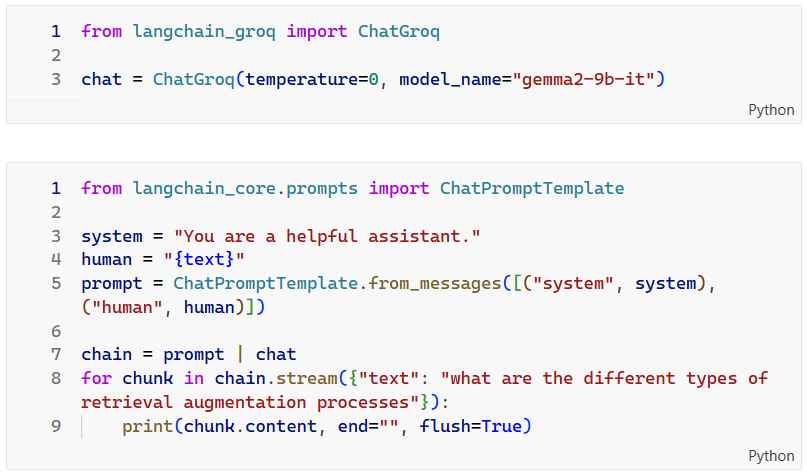
\includegraphics[width=\linewidth]{./figures/code-norag.png}
    \caption{Implementation of a question-answering LLM (No RAG)}
    \begin{flushleft}
        \small First, we start by initializing a chat model, Gemma-2 from GroqCloud, and instruct it to provide a helpful answer to a given question (what are the different types of retrieval augmentation processes).
    \end{flushleft}
\end{figure}
The response the chat model provided is demonstrated in the following illustration.
\begin{figure}[H]
    \centering
    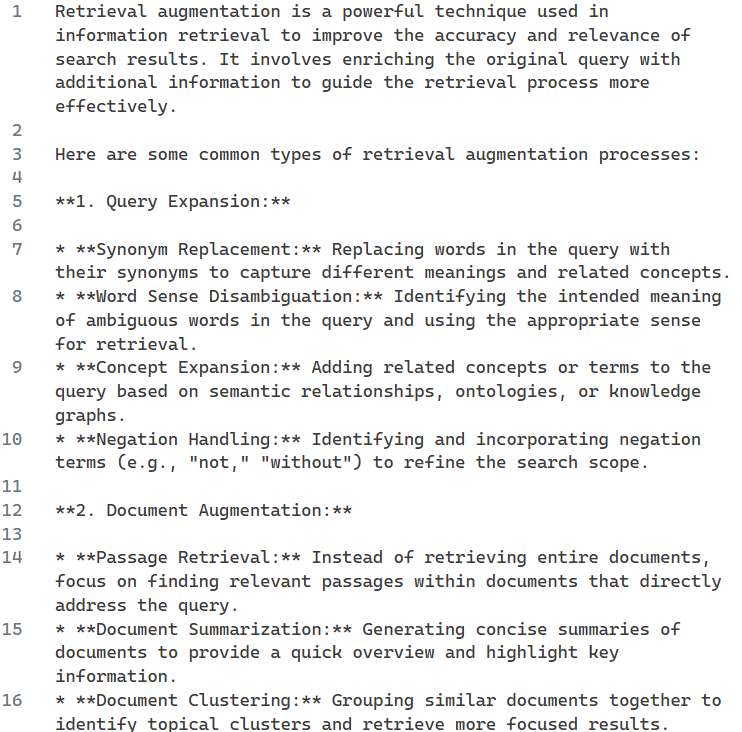
\includegraphics[width=\linewidth]{./figures/answer_norag.png}
    \caption{The response obtained from a LLM call directly}
\end{figure}
The example demonstrates the inconvenience of using an LLM when looking for a short and accurate response to a given query ("what are the different types of retrieval augmentation processes"). The generated answer is very long and clearly exhibits hallucination, as it is not accurate enough.\newline
The next section is about rectifying this inconvenience by implementing a RAG pipeline and providing relevant information from which the LLM base its response.

\section{Retrieval-augmented Generation Results}
\subsection{Data: Question and Answer}
We will need to load some data into the knowledge base. This information represents the ground truth on which we desire LLMs to base their answers.\newline
For this purpose, a \href{https://arxiv.org/abs/2312.10997}{PDF file from a research parper on Arxiv} will be uploaded as target data. Page 11 of this document contains the answer to our previous question, which we want to be automatically retrieved from the vector store.
\begin{figure}[H]
    \centering
    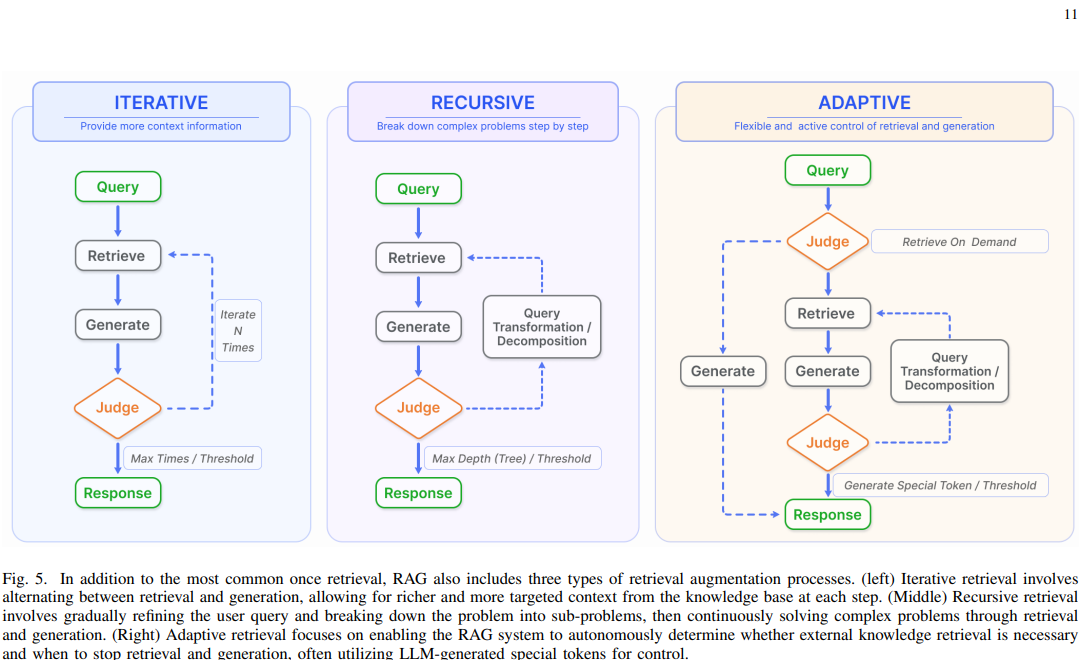
\includegraphics[width=\linewidth]{./figures/toberetrieved.png}
    \caption{The targeted context.}
    \begin{flushleft}
        \small This page from the PDF file contain clear answer to our question (3 types of retrieval augmentation processes: iterative, recursive, adaptive), explained in the caption.
    \end{flushleft}
\end{figure}
After having established a query to be asked to the model and its corresponding desired answer, we will now implement a simple RAG pipeline, similar to the one implemented in the system, with the same previous model (Gemma 2) to see the difference in generated answers.
\subsection{Knowledge Base initialization}
The first step is to load the PDF file into the knowledge base. For this purpose, we need to initialize a FAISS index with an embedding model (all-mpnet-base-v2), which will convert the information read from the file through PyMyPDFLoader to a numerical representation suitable for similarity search afterwards.
\begin{figure}[H]
    \centering
    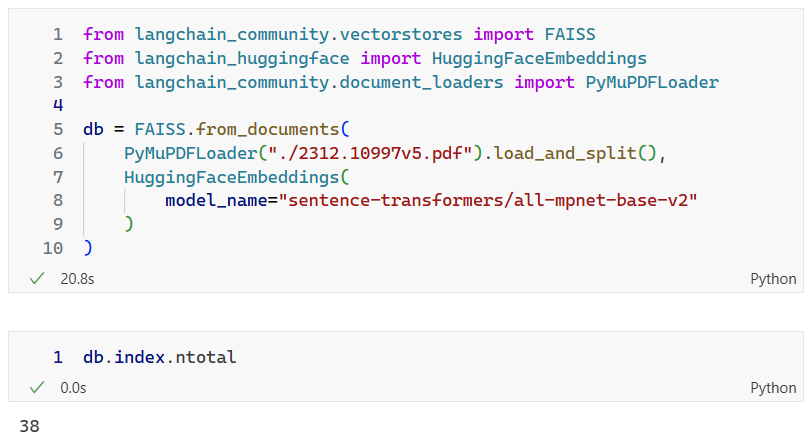
\includegraphics[width=\linewidth]{./figures/vectorstore_init.png}
    \caption{Vector Store initialization with data}
    \begin{flushleft}
        \small This sample vector store initialization included reading and loading the required PDF file from local storage, resulting in 38 chunks, which simplifies the process of retrieving and passing the most relevant chunks to the large language model later on.
    \end{flushleft}
\end{figure}
\subsection{Similarity Search dry run}
The following code imitates the retrieval phase in a complete RAG pipeline, providing an overview of the contents of the vector store and the results when some passages get retrieved.\newline
\begin{figure}[H]
    \centering
    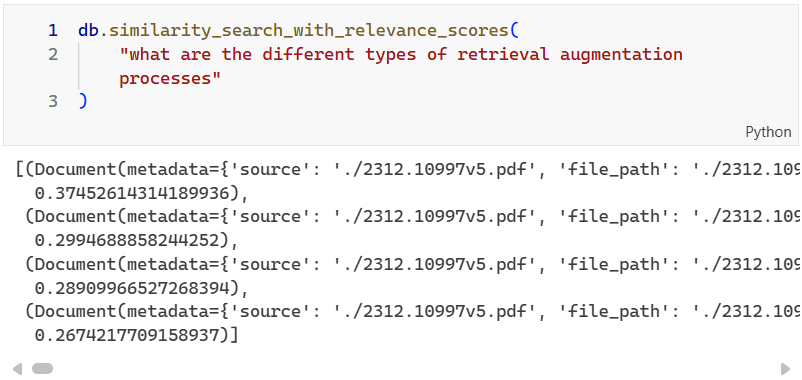
\includegraphics[width=\linewidth]{./figures/vectorstoresimilaritysearchwithscore_code.png}
    \caption{Retrieving relevant documents from the database}
    \begin{flushleft}
        \par The figure demonstrates a collapsed list of documents obtained from the database when applied to similarity search with the question "What are the different types of retrieval augmentation processes". The list is sorted by the cosine similarity score, and we can observe the passage we identified earlier as context in the third item.
    \end{flushleft}
\end{figure}
\begin{figure}[H]
    \centering
    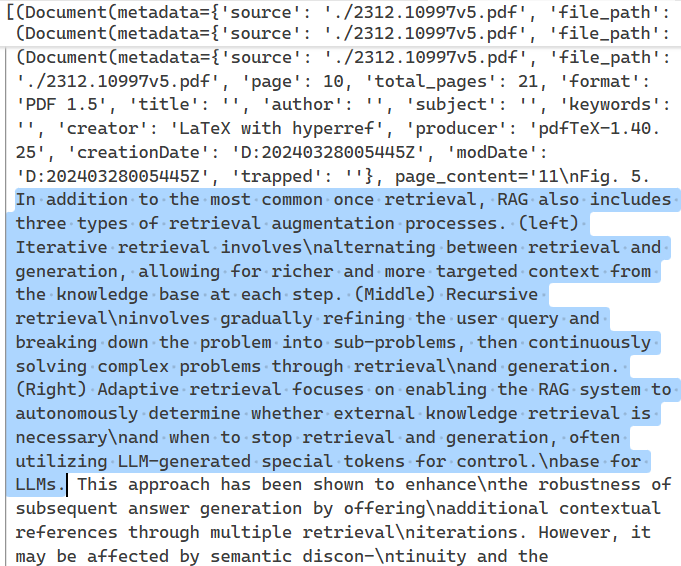
\includegraphics[width=\linewidth]{./figures/vectorstoresimilaritysearchwithscore_output.png}
    \caption{Output from similarity search}
    \begin{flushleft}
        \small The returned passages, as seen above, contain parsed text from the PDF file. As the vector store contain separate chunks, the result of running the previous code is a list containing document chunks, each with the textual content and some metadata that helps representing the whole documents through its chunks in a vector store. The highlighted text is the desired data that we want to pass to the LLM afterwards. This passage is returned 3rd on the list, with a score of 0.28.
    \end{flushleft}
\end{figure}
The results of retrieval, even though still optimizable (demonstrated later on in the answer sorting section), is satisfactory. Given a query, it is almost impossible to not retrieve the relevant passage outside the first 5 elements. This is because of the indexing strategy implemented in the vector store which allows to calculate the similarity between every chunk and the query to ensure most similar passages are retrieved effectively.\newline
These retrieved documents can now be integrated in a prompt and passed to the LLM to control the context of its generation process.
\subsection{Response with Retrieval-augmented Generation}
\begin{figure}[H]
    \centering
    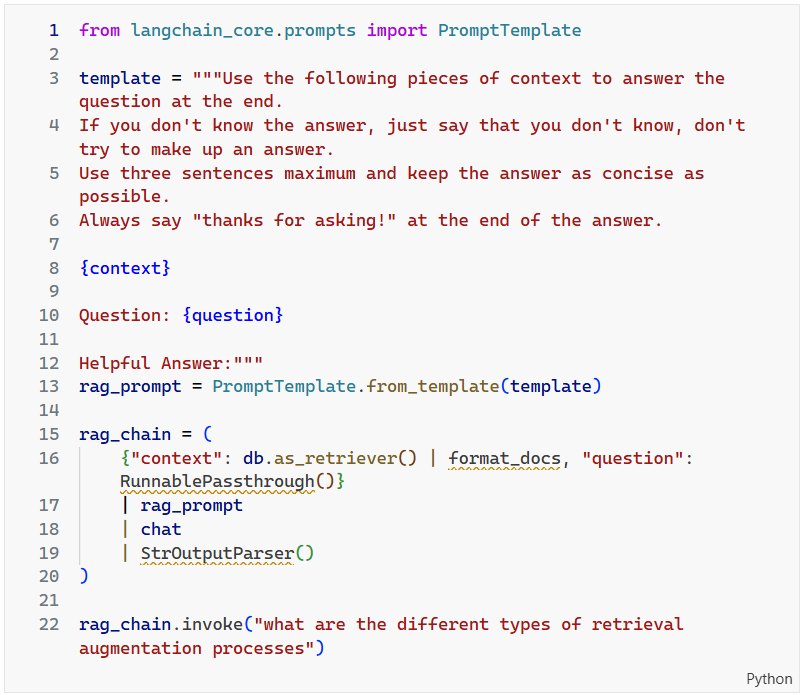
\includegraphics[width=.9\linewidth]{./figures/rag-code.png}
    \caption{Initialization of a simple RAG pipeline for testing}
    \begin{flushleft}
        \small The steps to initialize the RAG pipeline are: 1. set the prompt to support passing the context (retrieved documents) and question, along with instructing the model to only base its answer on the given context, 2. reconstructing the prompt by filling the variables (retrieving and formatting the context and the question), 3. passing the constructed prompt to the LLM (chat), 4. and finally transforming the LLM's response into a human readable format.
    \end{flushleft}
\end{figure}
Executing the previous code resulted in the desired output.
\begin{figure}[H]
    \centering
    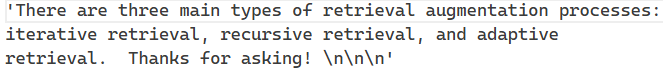
\includegraphics[width=\linewidth]{./figures/rag-answer.png}
    \caption{A simple RAG pipeline's generated answer}
\end{figure}
The response demonstrates how effective was the pipeline from transforming a long irrelevant answer into a very accurate and direct one.

\section{Answer Sorting}
The sorting algorithm allows for better answers to be more accessible by placing them at the bottom of less accurate ones (in our case where multiple LLMs attempt to generate the most suitable response given the same context).
To showcase how it affects the results page, here is a comparison between the positioning of generated answers from four different models (Claude 3.5 Sonnet, Command R+, Gemma-2 and Llama-3), using the previous example's question and data while employing the system's advanced RAG pipeline with its additional subprocess and phases.
\begin{figure}[H]
    \centering
    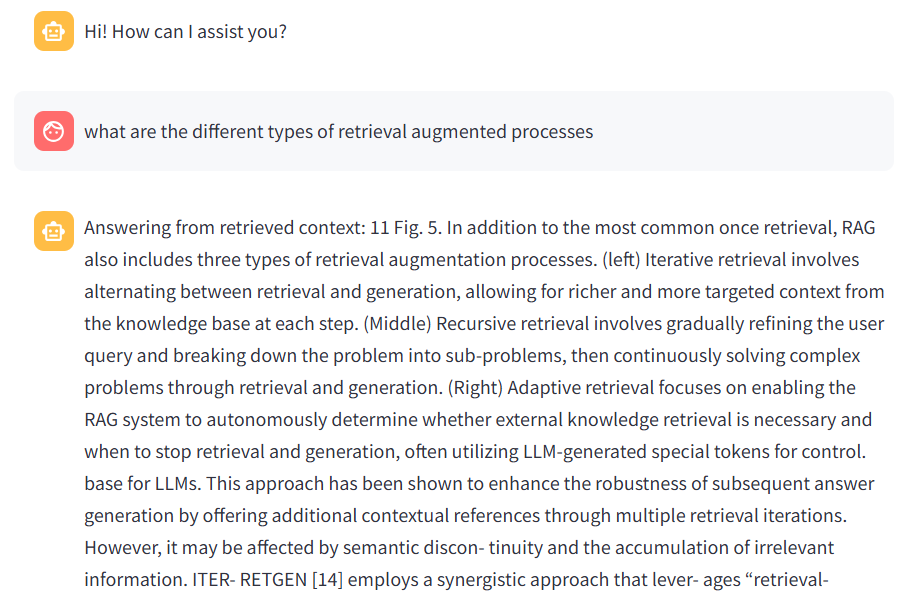
\includegraphics[width=\linewidth]{./figures/app-question.png}
    \caption{Prompting and retrieving context from the input question}
    \begin{flushleft}
        We can remark the effect of the re-ranking algorithm employed in the RAG pipeline, which prioritized the passage we identified in the first part of the "RAG results" previously.
    \end{flushleft}
\end{figure}
After the context gets retrieved from the selected vector stores, the LLMs generate answers based on its contents as shown below.
\begin{figure}[H]
    \centering
    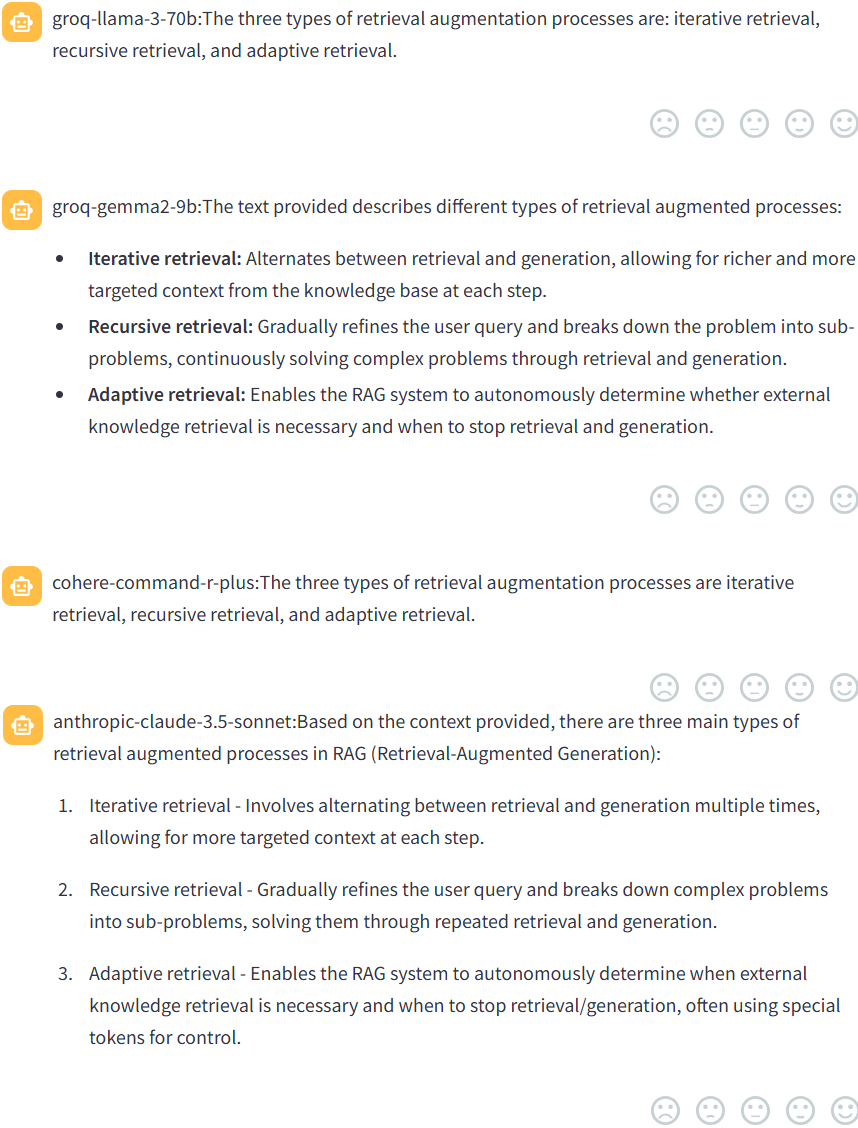
\includegraphics[width=.8\linewidth]{./figures/app-answers.png}
    \caption{Generated answers: not sorted}
\end{figure}
We can observe that the generated answers have clear differences. Some models perform better than others in certain cases, and this behavior alternates, meaning it is impossible to determine the best models for every use case. For this example, all the models generated relevant answers, but Claude and Gemma provided further accurate details. The results, however, are not sorted in any order, except the order of which the user has selected their preferred LLMs. It is possible that the more accurate responses get shadowed by less relevant ones (as the case with the Gemma-2 response in this example). Our goal for this app is to allow users to select the LLMs they prefer, while prioritizing better answers first automatically, which can be achieved by checking an option in the web interface to toggle the sorting algorithm.\newline
The following figure demonstrates the ranking of the previous answers to prioritize better quality results.\newline
The Gemma-2 and Claude-3.5 models performed better than the other models, providing more information extracted from the retrieved context, while Llama-3 and Command R+ did not use the available information from the context and generated more succinct answers.\newline
\begin{figure}[H]
    \centering
    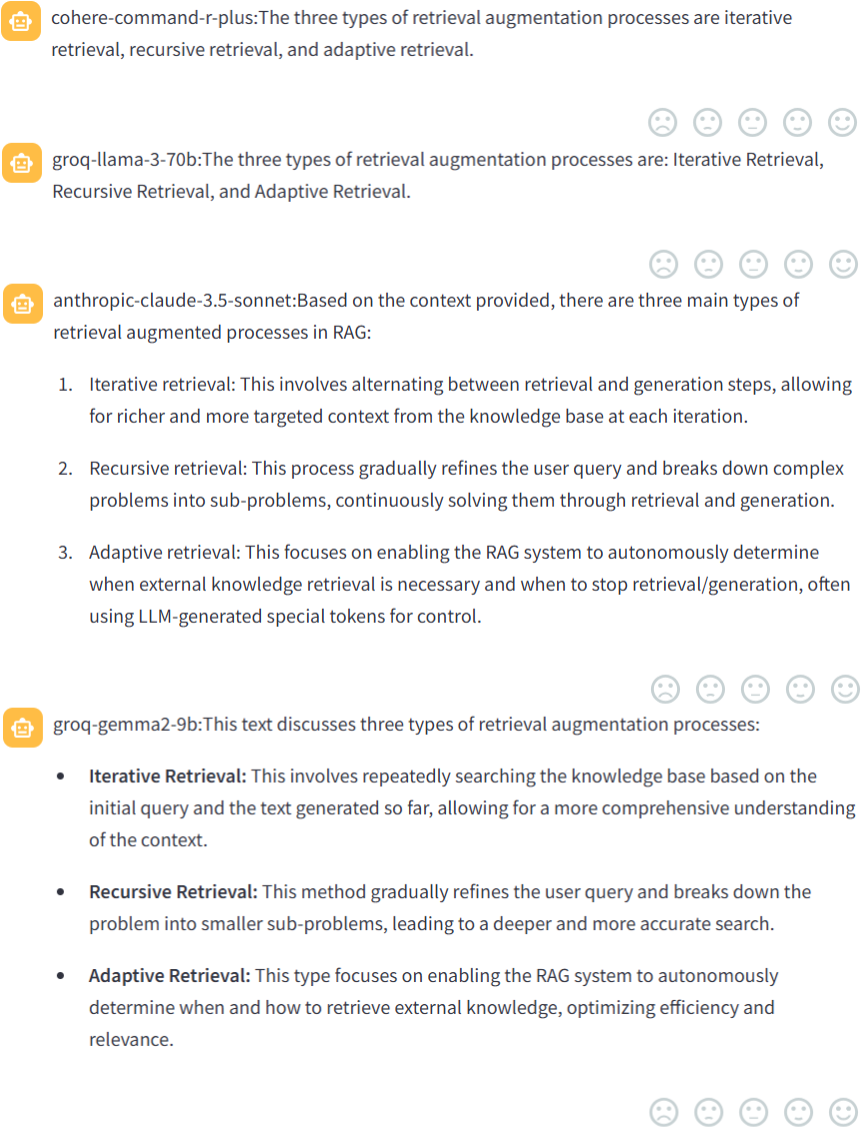
\includegraphics[width=\linewidth]{./figures/app-answers-sorted.png}
    \caption{Generated answers: sorted}
    \begin{flushleft}
        The ranking algorithm employed metrics specifically designed to evaluate RAG processes, measuring the consistency of the generated response against the given context, and assessing its pertinence to the original prompt.
    \end{flushleft}
\end{figure}

\section{Conclusion}
In conclusion, this project has demonstrated the efficacy of implementing and orchestrating a RAG pipeline to provide accurate and factual responses from a knowledge base. The employed retrieval phase methods can be used standalone to provide comparable results, but with the addition of a generation phase, we can leverage the NLP capabilities of LLMs to tune the responses to user queries and enrich results with valuable insights.